
%%%%%%%%%%%%%%%%%%%%%%%%%%%%%%%%%%%%%%%%%
% Short Sectioned Assignment LaTeX Template Version 1.0 (5/5/12)
% This template has been downloaded from: http://www.LaTeXTemplates.com
% Original author:  Frits Wenneker (http://www.howtotex.com)
% License: CC BY-NC-SA 3.0 (http://creativecommons.org/licenses/by-nc-sa/3.0/)
%%%%%%%%%%%%%%%%%%%%%%%%%%%%%%%%%%%%%%%%%

%----------------------------------------------------------------------------------------
%	PACKAGES AND OTHER DOCUMENT CONFIGURATIONS
%----------------------------------------------------------------------------------------

\documentclass[paper=a4, fontsize=11pt]{scrartcl} % A4 paper and 11pt font size

% ---- Entrada y salida de texto -----

\usepackage[T1]{fontenc} % Use 8-bit encoding that has 256 glyphs
\usepackage[utf8]{inputenc}
%\usepackage{fourier} % Use the Adobe Utopia font for the document - comment this line to return to the LaTeX default

% ---- Idioma --------

\usepackage[spanish, es-tabla]{babel} % Selecciona el español para palabras introducidas automáticamente, p.ej. "septiembre" en la fecha y especifica que se use la palabra Tabla en vez de Cuadro

% ---- Otros paquetes ----

\usepackage{url} % ,href} %para incluir URLs e hipervínculos dentro del texto (aunque hay que instalar href)
\usepackage{amsmath,amsfonts,amsthm} % Math packages
%\usepackage{graphics,graphicx, floatrow} %para incluir imágenes y notas en las imágenes
\usepackage{graphics,graphicx, float} %para incluir imágenes y colocarlas
\usepackage{subfigure} % subfiguras

% Para hacer tablas comlejas
%\usepackage{multirow}
%\usepackage{threeparttable}

%\usepackage{sectsty} % Allows customizing section commands
%\allsectionsfont{\centering \normalfont\scshape} % Make all sections centered, the default font and small caps

\usepackage{fancyhdr} % Custom headers and footers
\usepackage{pdflscape}

\pagestyle{fancyplain} % Makes all pages in the document conform to the custom headers and footers
\fancyhead{} % No page header - if you want one, create it in the same way as the footers below
\fancyfoot[L]{} % Empty left footer
\fancyfoot[C]{} % Empty center footer
\fancyfoot[R]{\thepage} % Page numbering for right footer
\renewcommand{\headrulewidth}{0pt} % Remove header underlines
\renewcommand{\footrulewidth}{0pt} % Remove footer underlines
\setlength{\headheight}{13.6pt} % Customize the height of the header

\numberwithin{equation}{section} % Number equations within sections (i.e. 1.1, 1.2, 2.1, 2.2 instead of 1, 2, 3, 4)
\numberwithin{figure}{section} % Number figures within sections (i.e. 1.1, 1.2, 2.1, 2.2 instead of 1, 2, 3, 4)
\numberwithin{table}{section} % Number tables within sections (i.e. 1.1, 1.2, 2.1, 2.2 instead of 1, 2, 3, 4)


\setlength\parindent{0pt} % Removes all indentation from paragraphs - comment this line for an assignment with lots of text

\newcommand{\horrule}[1]{\rule{\linewidth}{#1}} % Create horizontal rule command with 1 argument of height
\usepackage[breaklinks=true]{hyperref}

\usepackage[dvipsnames]{xcolor}
\usepackage{amssymb}
\usepackage{color}
\usepackage{listings}
\usepackage{upgreek} % para poner letras griegas sin cursiva
\usepackage{cancel} % para tachar
\usepackage{mathdots} % para el comando \iddots
\usepackage{mathrsfs} % para formato de letra
\usepackage{stackrel} % para el comando \stackbin
\lstset{ %
language=C++,                % elegir el lenguaje del código
stringstyle=\color{blue}\ttfamily,,
basicstyle=\normalsize\ttfamily,       % el tamaño del font a usar para el código
numbers=left,                   % dónde poner los números de línea 
numberstyle=\footnotesize,      % tamaño de font usados para los números de línea 
stepnumber=1,                   % el paso de numeración
numbersep=5pt,                  % distancia del numero de línea y la línea
backgroundcolor=\color{white},  % color de fondo, para usarlo hay que agregar  \usepackage{color}
showspaces=false,               % mostrar espacios en blanco ?
showstringspaces=false,         % subrayar espacios con cadenas?   
 showtabs=false,                 % mostrar taba usando cadenas? 
frame=single,           			% enmarcar el código?  
tabsize=2,          				% sets default tabsize to 2 spaces?
keywordstyle=\color{MidnightBlue}\ttfamily\bfseries,
commentstyle=\color{OliveGreen}\ttfamily,
morecomment=[l][\color{OliveGreen}]{\#},
captionpos=b,           % sets the caption-position to bottom?
breaklines=true,        % sets automatic line breaking?
breakatwhitespace=false,    % sets if automatic breaks should only happen at whitespace ?
title=\lstname,
escapeinside={\%*}{*)}          % if you want to add a comment within your code
}

\lstset{literate=
  {á}{{\'a}}1 {é}{{\'e}}1 {í}{{\'i}}1 {ó}{{\'o}}1 {ú}{{\'u}}1
  {Á}{{\'A}}1 {É}{{\'E}}1 {Í}{{\'I}}1 {Ó}{{\'O}}1 {Ú}{{\'U}}1
  {à}{{\`a}}1 {è}{{\`e}}1 {ì}{{\`i}}1 {ò}{{\`o}}1 {ù}{{\`u}}1
  {À}{{\`A}}1 {È}{{\'E}}1 {Ì}{{\`I}}1 {Ò}{{\`O}}1 {Ù}{{\`U}}1
  {ä}{{\"a}}1 {ë}{{\"e}}1 {ï}{{\"i}}1 {ö}{{\"o}}1 {ü}{{\"u}}1
  {Ä}{{\"A}}1 {Ë}{{\"E}}1 {Ï}{{\"I}}1 {Ö}{{\"O}}1 {Ü}{{\"U}}1
  {â}{{\^a}}1 {ê}{{\^e}}1 {î}{{\^i}}1 {ô}{{\^o}}1 {û}{{\^u}}1
  {Â}{{\^A}}1 {Ê}{{\^E}}1 {Î}{{\^I}}1 {Ô}{{\^O}}1 {Û}{{\^U}}1
  {œ}{{\oe}}1 {Œ}{{\OE}}1 {æ}{{\ae}}1 {Æ}{{\AE}}1 {ß}{{\ss}}1
  {ű}{{\H{u}}}1 {Ű}{{\H{U}}}1 {ő}{{\H{o}}}1 {Ő}{{\H{O}}}1
  {ç}{{\c c}}1 {Ç}{{\c C}}1 {ø}{{\o}}1 {å}{{\r a}}1 {Å}{{\r A}}1
  {€}{{\EUR}}1 {£}{{\pounds}}1
  {ñ}{{\~n}}1
}

\hypersetup{
    colorlinks=true,
    linkcolor=black,
    filecolor=magenta,      
    urlcolor=blue,
    pdftitle={EC: Práctica 3 - Mario Rodríguez Ruiz},
    bookmarks=true,
    citecolor=blue,
}





%----------------------------------------------------------------------------------------
% DOCUMENTO
%----------------------------------------------------------------------------------------

\begin{document}
	
{\LARGE Desactivación Bomba de Javier Bueno \par}
\vspace{5mm}
{\large Estructura de Computadores - Grupo C3 \par}
\vspace{3mm}
{\large \textit{Mario Rodríguez Ruiz} \par}	
	
	
%----------------------------------------------------------------------------------------
%	Cuestión 1
%----------------------------------------------------------------------------------------

\section{Contraseña}

Para averiguar la contraseña se ha utilizado el depurador \textbf{DDD} realizando los siguientes pasos:
\\

En primer lugar se ha puesto un punto de ruptura en la llamada a \textbf{fgets}, que es cuando se le pide al usuario por pantalla que ingrese una contraseña.\\

Una vez funcionando el programa y detenido ahí (como se ve en la Figura \ref{fig:figura1}) se ha metido una contraseña al azar (\textbf{hola}) para avanzar.

\begin{figure}[H]
	\centering
	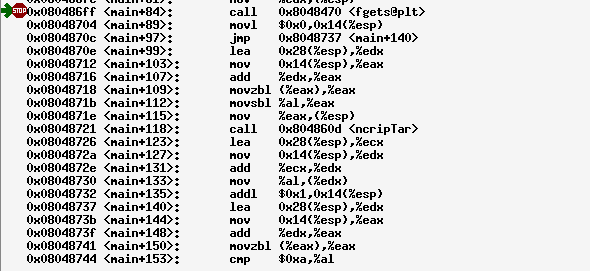
\includegraphics[scale=0.9]{capturas/figura1.png} 
	\caption{Comienzo de la depuración desde DDD} 
	\label{fig:figura1}
\end{figure}

Una vez introducida la contraseña por consola, el programa entra
en una función llamada \textbf{ncripTar} para modificar todos los componentes de la cadena.\\

Se puede demostrar que se han cambiado todos éstos viendo el contenido del registro que contiene ahora la contraseña modificada justo después de salir de \textbf{ncripTar}.
\\

Para ello se ha utilizado la herramienta \textbf{Data}$ \rightarrow $\textbf{Memory}, volcando el contenido de \textbf{\%edx} en pantalla.\\

En la Figura \ref{fig:figura2} puede verse que el valor de la cadena después del "\ encriptado "\ es \textbf{']daV' }. Esto supone que se ha realizado una \textbf{resta con valor 11} sobre cada uno de los componentes de la cadena.
\begin{figure}[H]
	\centering
	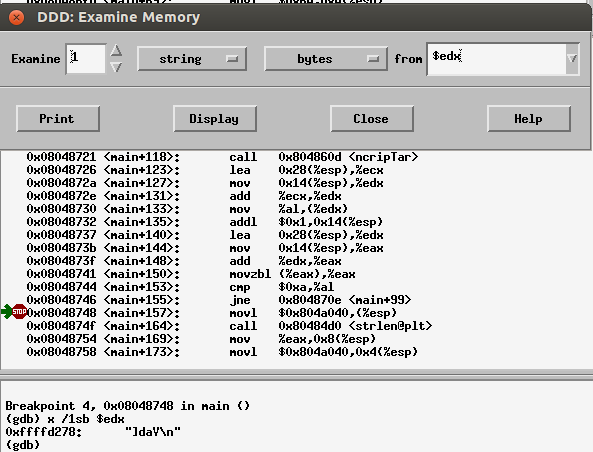
\includegraphics[scale=0.9]{capturas/figura2.png} 
	\caption{Contraseña introducida modificada} 
	\label{fig:figura2}
\end{figure}



Ahora tan solo falta encontrar una supuesta contraseña con la que se compare la que se ha introducido. Lo que se hace es volcar el contenido del registro que se encuentra justo antes de la comparación de ambas, ya que es ahí donde se encuentra liberado. Este volcado se consigue mediante la misma herramienta que en el caso anterior (\textbf{Data}$ \rightarrow $\textbf{Memory}), pero cambiando el valor del registro, que será: \textbf{0x804a040}.
\begin{figure}[H]
	\centering
	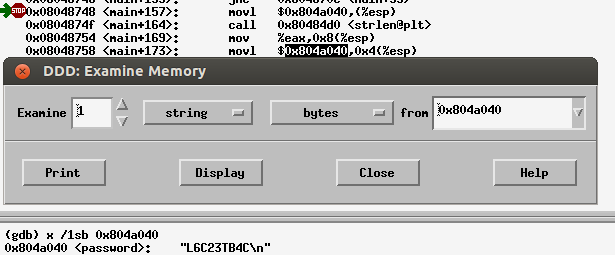
\includegraphics[scale=0.9]{capturas/figura3.png} 
	\caption{Valor de la contraseña a buscar encriptada} 
	\label{fig:figura3}
\end{figure}

El valor que aparece en la Figura \ref{fig:figura3} (\textbf{L6C23TB4C}) se trata de la contraseña que se está buscando pero con el único inconveniente de estar cifrada (mediante la función que se vio anteriormente: \textbf{ncripTar}).

Su valor original se obtiene al hacer la función inversa, es decir, sumándole 11 a cada componente de la cadena. \\

Contraseña: \textbf{WAN=>\_M?N}
\newpage

%----------------------------------------------------------------------------------------
%	
%----------------------------------------------------------------------------------------

\section{Código}
Para averiguar la contraseña se ha utilizado el depurador \textbf{DDD} realizando los siguientes pasos:
\\

Llegando a la sección del programa que se encarga de procesar y validar el código, se ha puesto un punto de ruptura en esta parte para futuros intentos.\\

En este punto el programa vuelve a solicitar datos, en este caso los correspondientes al código. El código introducido como prueba es \textbf{1111}, tal y como se ve en la Figura \ref{fig:figura4} en el estado de registros (\textbf{Status}$ \rightarrow $\textbf{Registers})
\begin{figure}[H]
	\centering
	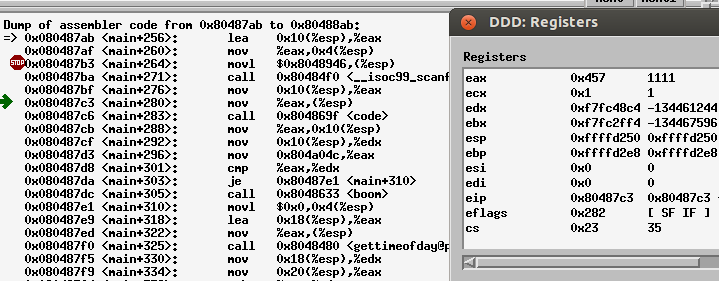
\includegraphics[scale=0.8]{capturas/figura4.png} 
	\caption{Status Registers desde DDD para el código} 
	\label{fig:figura4}
\end{figure}

Siguiendo el trascurso del programa mediante \textbf{Nexti} y manteniendo la ventana del estado de registros abierta, se puede comprobar cómo el valor del código introducido ha sido modificado. Ahora su valor es de \textbf{1090} como presenta la Figura \ref{fig:figura5}.

\begin{figure}[H]
	\centering
	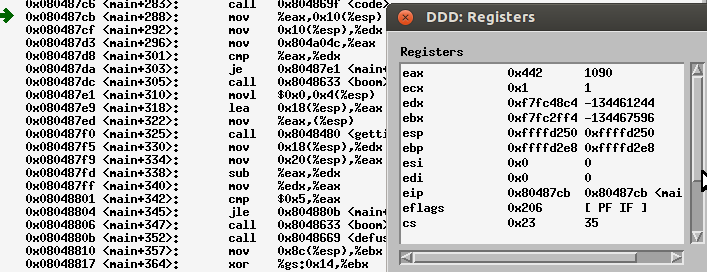
\includegraphics[scale=0.8]{capturas/figura5.png} 
	\caption{Status Registers desde DDD para el código} 
	\label{fig:figura5}
\end{figure}

Al parecer no se realiza ninguna modificación más sobre el código introducido por consola, porque ya se ha llegado a la comparación final de valores antes de retornar a main. Se puede deducir que lo único que se hace para cambiar el valor es la \textbf{resta de} \textbf{21} sobre éste.

\begin{figure}[H]
	\centering
	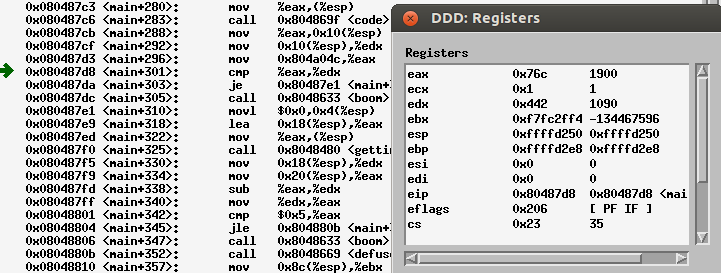
\includegraphics[scale=0.8]{capturas/figura6.png} 
	\caption{Status Registers desde DDD para el código} 
	\label{fig:figura6}
\end{figure}

Dicha comparación puede visualizarse en la Figura \ref{fig:figura6}, donde se encuentran ambos valores en la ventana del estado de registros:

El código introducido por consola y modificado posteriormente se encuentra en el registro \textbf{\%edx} con el valor anteriormente mencionado (\textbf{1090}) y el valor original del código con cifrado está en \textbf{\%eax} con \textbf{1900} como contenido.\\

Por tanto, para terminar con el proceso lo único que hay que hacer es realizar la modificación inversa sobre \textbf{1900} (\textbf{suma de 21}).
\\

Código: \textbf{1921}


\section{Prueba final}

En la Figura \ref{fig:figura7} se presenta la prueba de desactivación de la bomba del compañero Javier Bueno López con contraseña \textbf{WAN=>\_M?N} y código \textbf{1921}.

\begin{figure}[H]
	\centering
	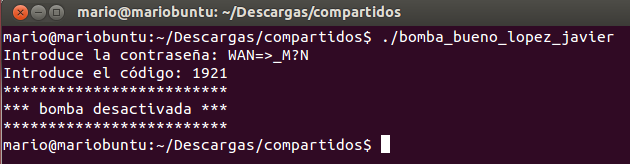
\includegraphics[scale=0.9]{capturas/figura7.png} 
	\caption{Prueba de desactivación} 
	\label{fig:figura7}
\end{figure}
%----------------------------------------------------------------------------------------
%	Referencias
%----------------------------------------------------------------------------------------
%------------------------------------------------

\bibliography{citas} %archivo citas.bib que contiene las entradas 
\bibliographystyle{plain} % hay varias formas de citar

\end{document}
